
\chapter{Monophoton Analysis [TODO WESLEY COMMENTS] }\label{sec:lgxc}

While studying the Standard Model process \ppwbb is a means
 for probing the physics associated with jets,
 hadronization and the modeling of the proton 
 parton distribution function, the monophoton analysis,
 charactarized by a final state consisting of \gmet 
 is also of interest for validating SM and possibly extending it
 via the search for dark matter (DM).
One interpretation presented in this work
 is the SM process \ppzgnng  in which the \met is interpreted as coming from the
 invisible decay of the \z boson, \znn.
As discussed in Section \ref{sec:lgproduction},
 it is also possible to extend this cross section measurement
 into a dark matter search under the interpretation 
 that the \met arises from the 
 annihilation of incoming particles into DM 
 and the $\gamma$ is initial state radiation 
 recoiling against thie process. 
Under this interpretation, limits are set on the
 cross section of DM as a function of the 
 mediator mass for vector and axiel-vector models. 
This analysis is performed using protons colliding at
 \s 13 \TeV provided by the LHC and detected by
 the CMS detector.

\section{Previous Measurements}

A similar search was performed by the ATLAS experiment~\cite{Aaboud:2016uro}
 using 3.2\fbinv of pp collision data at \s 13 \TeV
 collected in 2015, and no evidence for new physics was found. 
The fiducual cross section for 
 the monophoton final state with photon $\etg > 150 \GeV$
 and $\met > 150 \GeV$ was measured to be below 17.8 \fbinv.
A prior search~\cite{Khachatryan:2014rwa} at the CMS 
 experiment used the LHC run 1 data collected in 2012 at
 \s 8 \TeV, and set a cross section upper limit for the monophoton final
 state with photon $\etg > 145\GeV$ and $\met > 140\GeV$ at 13 \fbinv. 

\section{Event Selection}\label{subsec:lgevent_selection}

The sample of data analyzed was collected using 
 a trigger that requires at least one photon
 candidate with $\etg > 165 \GeV$ and 
 requires at least 90\% of the energy deposited in 
 the calorimeters to be deposited in the ECAL
 to reject jets. 
This trigger is 98\% efficient at selecting photons
 which pass the other analysis selections.
Events passing the trigger are further required to
 have at least one photon with $\etg > 175\GeV$
 in the barrel fiducial region ($\abs{\eta} < 1.44$).

To distinguish photons from electrons, which leave a similar
 signature of energy deposits in the ECAL and HCAL,
 candidate photons are required
 to not have any associated track seeds in the pixel detector. 
To distinguish photons from jets, selections based on calorimetric
 information and isolation are applied. 
The fraction of energy deposited in the ECAL compared 
 to the total deposit in the calorimeters
 is tighened relative to the trigger to be 95\%
 and the shower shape variable in the $\eta$ direction,
  $\sieie$, described in Section \ref{sec:sieie},
 is required to be $\sieie < 0.0102$. 

  %Ref.~\cite{Khachatryan:2015iwa},
%encodes the width of the electromagnetic shower in the $\eta$
%direction, which is generally larger in showers from hadronic
%activity. 

For a photon object to be considered isolated,
 scalar sums of the transverse momenta of PF charged hadrons, neutral
 hadrons, and photons within a cone of $\Delta R = \sqrt{(\Delta
  \eta)^2 + (\Delta \phi)^2} < 0.3$ around the candidate photon must
 individually fall below bounds defined for 80\% signal
 efficiency. 
Only the PF candidates that do not overlap with the 
 electromagnetic shower of the candidate photon are used in the 
 isolation sums.

Because photon objects are not reconstructed from tracks,
 there is an ambiguity in identifying the collision
 vertex that the photon originates from in the presence 
 of pileup collisions.

Association of a vertex to the photon candidate impacts the photon in two ways. 
First, the photon momentum direction is given by a straight line connecting
the ECAL cluster position and the vertex. Second, the isolation sum 
using the PF charged hadrons include only the candidates whose tracks
are associated to the vertex. While the first effect is minor and is
not relevant for this analysis, the second will cause photon
candidates that are actually non-isolated to appear otherwise, if the 
vertex is misassigned.  In practice, photon momentum is always
computed with respect to the primary vertex, defined as the vertex
with the highest $\sum \pt^2$ of the associated tracks.  However, for 
the charged hadron isolation sum, all vertices are considered, and the 
maximum value of the isolation sum is used as a conservative estimate
of the true isolation sum (worst isolation).

To reduce the contribution of backgrounds arising from 
 occurances in the CMS detector which did not originate from
 collisions, the pulse in the seed crystal of the photon cluster
 is required to be within $\pm 3\ns$ of the time expected
 for particles from a collision, and the cluster must not
 be so narrow that it is consistent with a cluster formed by a single crystal.  
To reduce contamination from beam halo, the ECAL
 crystals not  associated with the photon candidate are 
 examined for evidence of the passage of a minimum-ionizing
 particle roughly parallel to the beam axis (beam halo tag).
If at least  4.9 \GeV of energy is found deposited along
 this trajectory, the event is rejected.

%To further
%suppress the beam halo background, possible paths of halo muons that
%run through each photon candidate are considered, and the total energy
%deposit in the ECAL along the path that is the most compatible with
%the halo hypothesis is required to be below a threshold, defined to
%achive 95\% efficiency over prompt photons.

%The missing transverse momentum (\ptvecmiss) is defined by the
%magnitude of the vector sum of the transverse momenta of all PF
%candidates in the event. The magnitude of \ptvecmiss is \met. Jets are
%%also formed from PF candidates, and are clustered using the anti-\kt
%algorithm~\cite{Cacciari:2008gp} with a distance parameter of 0.4. Jet
%energies are calibrated to account for pileup effects and detector
%response.

The candidate events are required to have \met $> 170$\GeV.
%after
%adjusting \ptvecmiss for the difference between simple momentum sums
%of PF candidates and calibrated jet momenta. 
The azimuthal opening
angle between the candidate photon and $\vmet$ is required to be
greater than 2 to ensure that the main source of \met is not photon
energy mismeasurement.  

Because jet energy mismeasurement can also
give rise to \met, events are rejected if the minimum azimuthal opening
angle between $\vmet$ and up to four leading jets (\minDphiMETj) is
less than 0.5.

Finally, events are also vetoed if they contain 
 a charged lepton (an electron or a muon) with $\pt >
10\GeV$ that is separated from the photon by $\Delta R > 0.5$.

After applying all of the selection criteria, 77 candidate events are 
found in data.

\section{Estimation of Contributions}

The dominant SM processes contributing to this 
 phase space are the associated productions of a \z
 or \w boson with a high-energy photon. 
If the \z boson decays into a  neutrino-antineutrino pair, 
 the final state exhibits a high-\et photon and large
 missing transverse energy. 
Similarly, if the \w boson decays into a lepton-neutrino
 pair and  the lepton is outside of the detector acceptance
 or fails reconstruction, the event appears to be \gmet.
 Together, these two processes account for approximately
  75\% of the simulated events and are
 estimated using Monte Carlo (MC) simulations. 
Hard-scattering events are generated with \MGfiveAMC\
  version 2.2~\cite{Alwall:2014hca} at leading order (LO) in QCD,
 with  \NNPDFthree LO ($\as = 0.130$) as the parton distribution function.
Parton shower and hadronization is performed by \PYTHIA{}8.2~\cite{Sjostrand:2014zea}.
Generated particles are processed through the full \GEANT-based simulation of the CMS 
 detector \cite{GEANT, GEANTdev} and event reconstruction used for data. 
Minimum-bias simulations are overlaid to model pileup interactions.

 \subsection{Reweighting}\label{subsubsec:lg_reweighting}
To account for differences arising from imperfect modeling of the data in
 the simulation, a total correction factor $\rho$ of $0.99\pm0.06$ is applied to all 
 MC-based  estimates. 
This is the product of individual correction factors taken as the
 ratios of the efficiencies measured in data and in simulation. 
They include
 $0.99\pm0.016$ for photon identification measured using \zee events,
 $1.00\pm0.0246$ for pixel seed measured using \zee events, and
 $1.00\pm0.05$ for worst isolation, beam halo tag and lepton veto measured using \zgnng events.
Generated samples are then weighted event by event with a product of two factors. 
The first factor matches the distribution of the generator-level photon
 \pt to that calculated at next-to-next-to-leading order (NNLO) in QCD using the 
 \DYRes~\cite{Catani:2015vma} calculator.
The second factor, taken from
 Refs.~\cite{Denner:2014bna,Denner:2015fca}, further corrects this distribution
 to account for electroweak next-to-leading order (NLO) effects. 

 \subsection{\vg Estimates}
After accounting for event selection efficiency difference between data and MC,
 respectively $42.1 \pm 6.3$ and $10.7 \pm 1.5$ events are estimated
 from \zgnng\ and \wglng. 
Four sources of systematic uncertainty on \zg and \wg estimates are considered:
 PDF and scale uncertainties, which are 5.37\% and 8.9\% respectively;
 electroweak correction uncertainties,
 where the full correction is conservatively taken as the uncertainty
 which is 11\% for \zg and 7\% for \wg;
 scale factors, which are 6\%;
 and the sytematic uncertainty due to jet/\met/$\gamma$ energy scale and pileup, which is 6.2\%. 
%To gain confidence in the estimates from simulation, control regions
% dominated by the various backgrounds and having negligible
% contributions from the signal, are defined in the data. 
As a crosscheck, the total contribution from \zgnng is estimated
 in data using a sample of \zgllg candidates,
 where the leptons from the decay of the Z boson are removed and considered as
 \met~\cite{monojet2014}. 
This provides an estimate of $64.6 \pm 17.6$, 
 where the uncertainty is dominated by the size of the sample.

 \subsection{Elecron Mis-ID}
The most important SM background comes from events where
 electrons are misidentified as photons, mainly in the \wen process. 
Seeding efficiency in the pixel detector for
 electron tracks is $\epsilon = 0.982 \pm 0.004$ for
 electrons with $\pt > 100\GeV$. 
This efficiency is measured in data using the
 tag-and-probe method~\cite{Khachatryan:2010xn} on \zee events,
 and is verified with MC simulation. 
Electrons from \w\ boson decay that are not seeded
 appear as isolated photons accompanied with large \met from the escaping neutrino. 
This class of events is modeled by an electron proxy event sample
 selected in data using criteria that are identical to those described in 
 Sec.~\ref{subsec:lgevent_selection}, except the photon candidate is required to have
a pixel seed. 
The number of electron proxy events is then scaled by
 $(1-\epsilon)/\epsilon$ to yield an estimated contribution of $7.4 \pm 1.2$ from
 electron misidentification events. 
The dominant uncertainty in the 
 estimate is the statistical uncertainty in the tag-and-probe fit, 
 and is assessed by generating a large ensemble
 of toy dielectron mass distributions
 on which the fit procedure is repeated. 
The standard deviation of the number
 of \zee events obtained from the fits is then propagated
 to the uncertainty in $\epsilon$.

 \subsection{Non-collision Backgrounds}
Non-collision backgrounds,  from  things such as detector noise,
 cosmic rays, and beam halo, are estimated from the time distribution of the cluster seeds
 since each process exhibits a disctintive time distribution when the cluster is
 in the ECAL barrel. 
Templates for anomalous signals, cosmic ray muons, and beam halo events
 are obtained by inverting the shower shape and beam halo tag requirements,
 and are fitted to the timing distribution of the candidate sample.
The only nonnegligible residual contribution to the candidate sample
 is found to arise from the beam halo, with an estimated $5.9\pm4.7$ events,
 where the uncertainty is from the template fit. 
%As a cross-check, a fit to the azimuthal angle ($\phi$) distribution of the candidate
% sample is performed. 
%Beam halo EM showers are observed to concentrate around
%$\phi \sim 0,\pi$, while all other (collision-origin) processes should yield
%photons that are uniformly distributed in $\phi$. This cross-check estimates
%the number of beam halo events in the signal sample to be less than 4.4 at 95\%
%confidence level.

 \subsection{Minor SM Processes}
The SM processes \wlng, \zllg, $W(l\nu)$ and $\gamma+jets$
 are generated with \MADGRAPH{}5$\_aMC@NLO$ at LO~\cite{Madgraph_new}
 with up to 2 jets and then
 processed with \PYTHIA6.426 generator~\cite{Pythia6} for showering and hadronization,
 with the \NNPDFthree LO($\as = 0.130$) parton distribution function.
The total background expectation from these processes is $3.05\pm 0.67$ events,
 where the uncertainty includes the statistical and systematic uncertainty due
 to scale factor and jet/\met/$\gamma$ energy scale.


 
\section{Results}

After applying our full selection criteria,we observe 77 events in 2.32 fb$^{-1}$ of data.
Table~\ref{tab:BkgSummaryC}
% ~\ref{tab:BkgSummaryC1} 
shows the estimated number of events and uncertainty from each background for the full 2015 run.


The \pt spectrum and particle flow \met of the full combination of our selected candidate events and estimated backgrounds can be seen in Figure \ref{fig:ptmetstack}
and the \pt/\met and number of jets distrbution is shown in Figure \ref{fig:ptmetstack1}.
%Likewise, Figure~\ref{fig:ratio_stack} and Figure~\ref{fig:addplots} shows the jet \pt, nvertices and $E_{T}^{\gamma}$/\met, $E_{T}^{\gamma}$/ jet \pt  for our selected candidate events and estimated backgrounds for the full candidate selection.
%Since data are compatible with the standard model expectation, upper limits on new physics processes cross
%sections are set.

\begin{figure}[htb]
\caption[Distributions of \pt and \met in the \pploneg analysis]
 {The photon \pt and \met\ distribution for the candidate sample,
  compared with estimated contributions from SM backgrounds, 
  here QCD$\gamma$ refers to $\gamma$+jet background and the
  background uncertainity includes statistical and systematic error. }
\centering
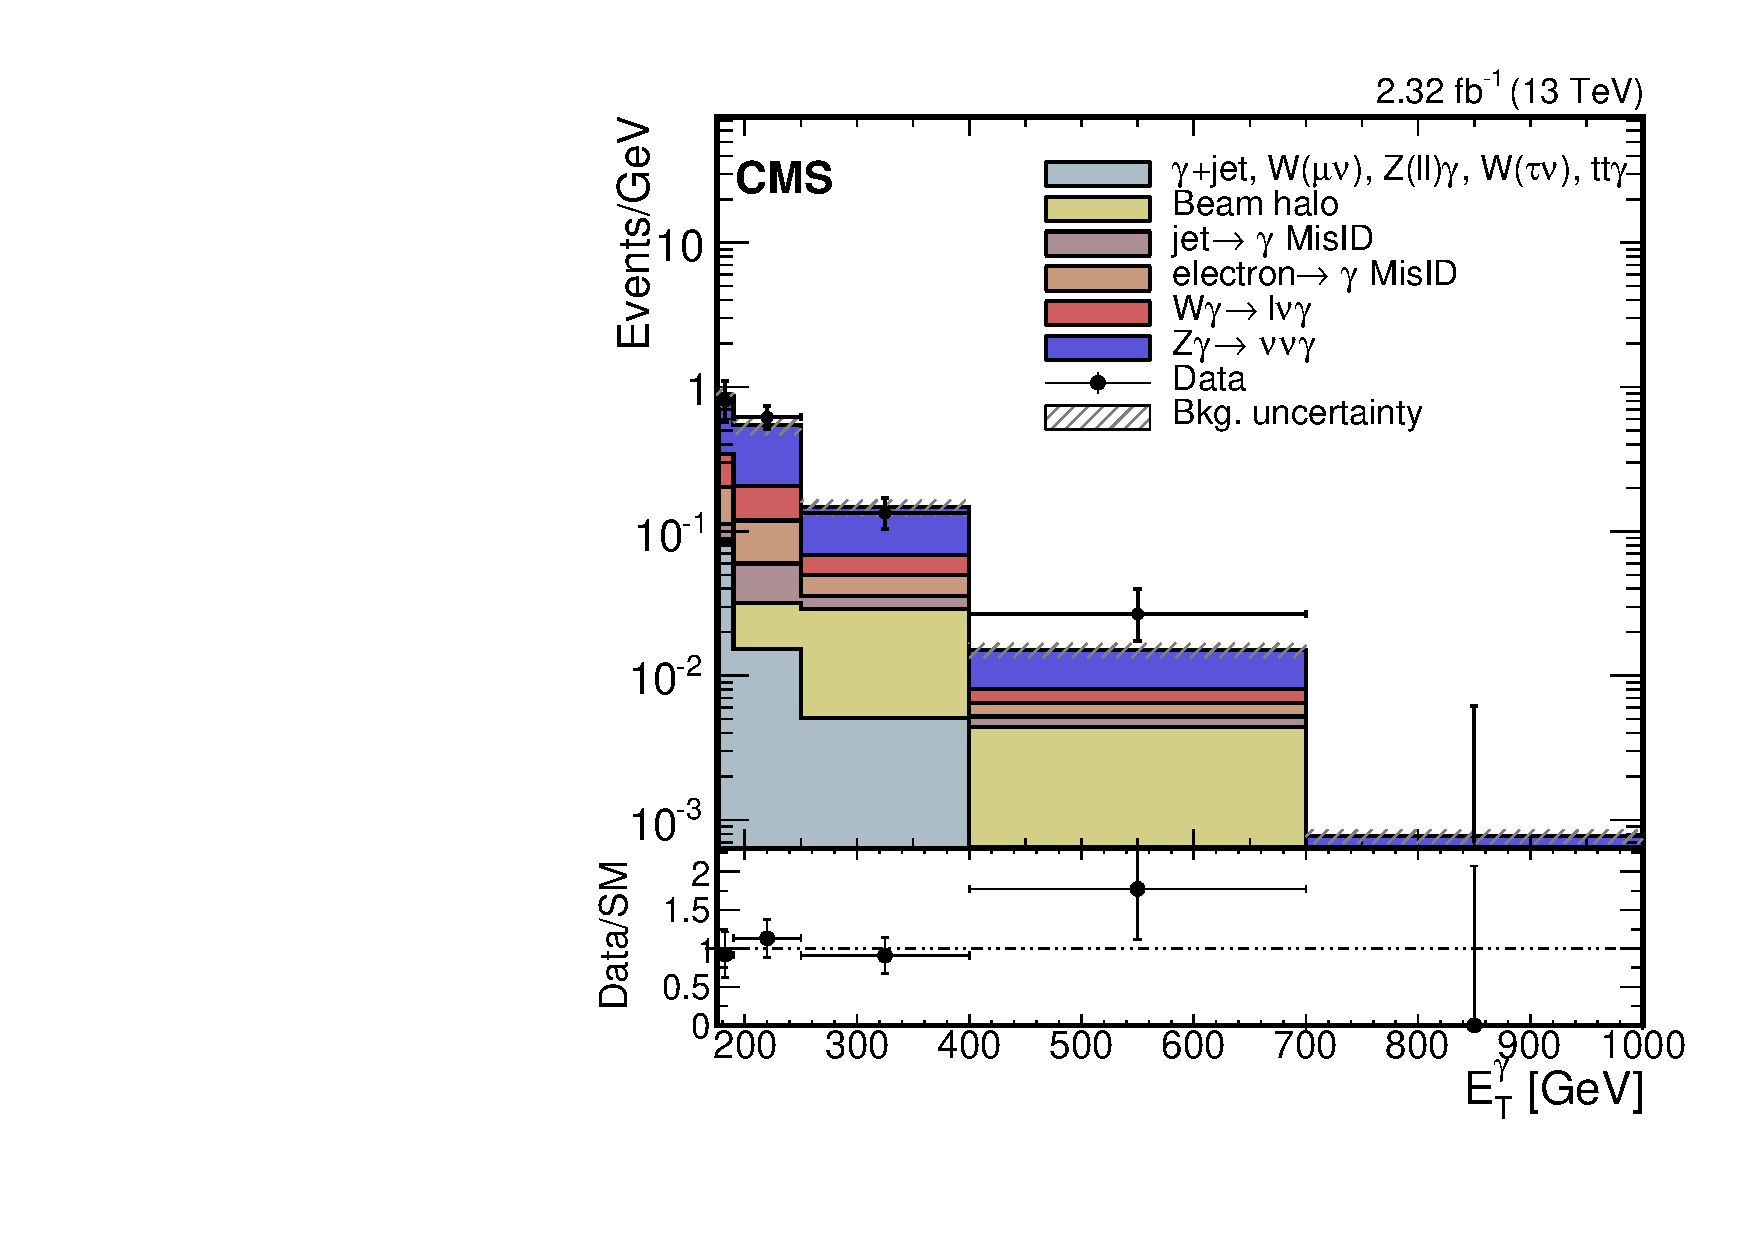
\includegraphics[width=8cm,height=8.0cm]{/Users/rhombus/CMS/Thesis/thesis/pdfs/lgxc/fromb/photon_pt8.pdf}
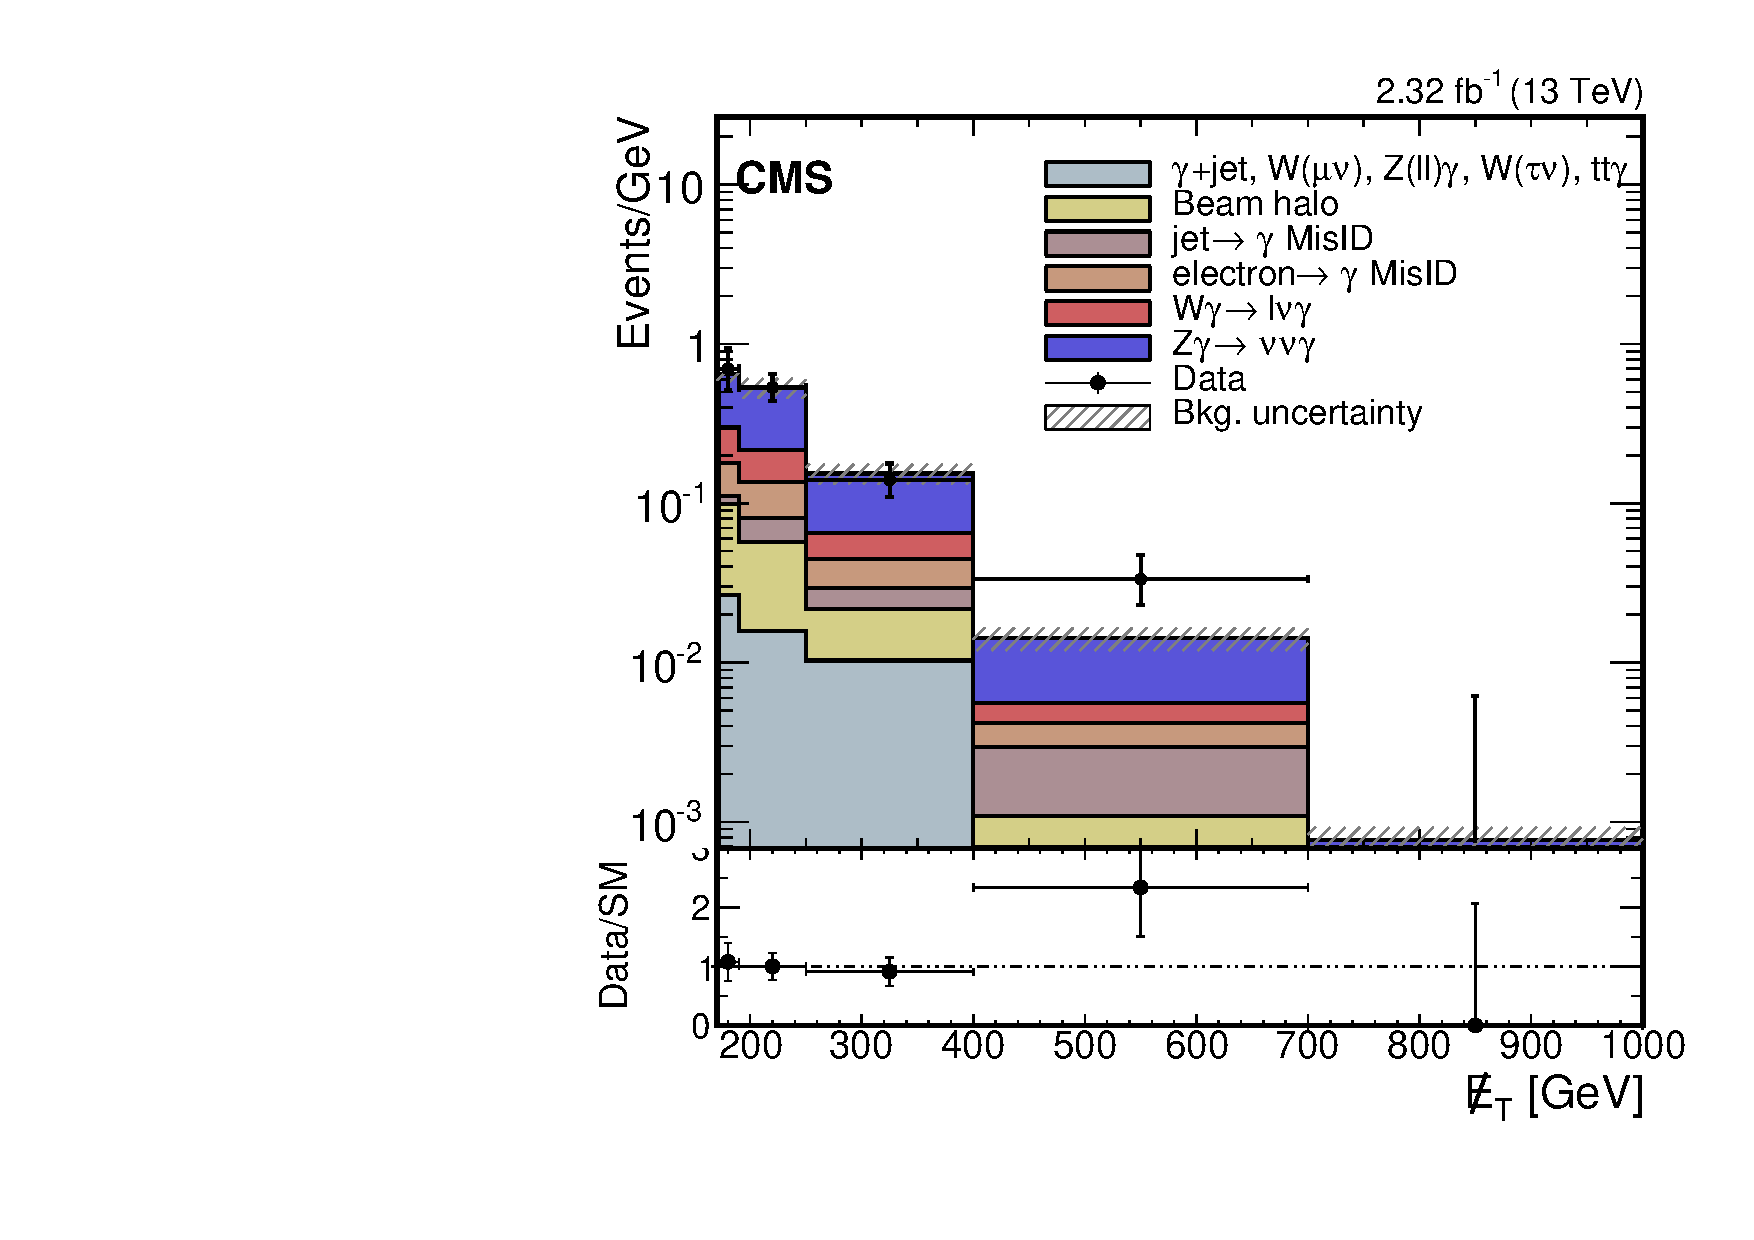
\includegraphics[width=8cm,height=8.0cm]{/Users/rhombus/CMS/Thesis/thesis/pdfs/lgxc/fromb/met8.pdf}
\label{fig:ptmetstack}
\end{figure}


\begin{figure}[!h]
\caption[Distributions of \pt/\met and $n_\mathrm{jets}$ in the \pploneg analysis]{
 The photon \pt/\met\ and number of jets distribution for the candidate sample, 
 compared with estimated contributions from SM backgrounds.
 The  background uncertainity shown includes statistical and systematic errors. }
\centering
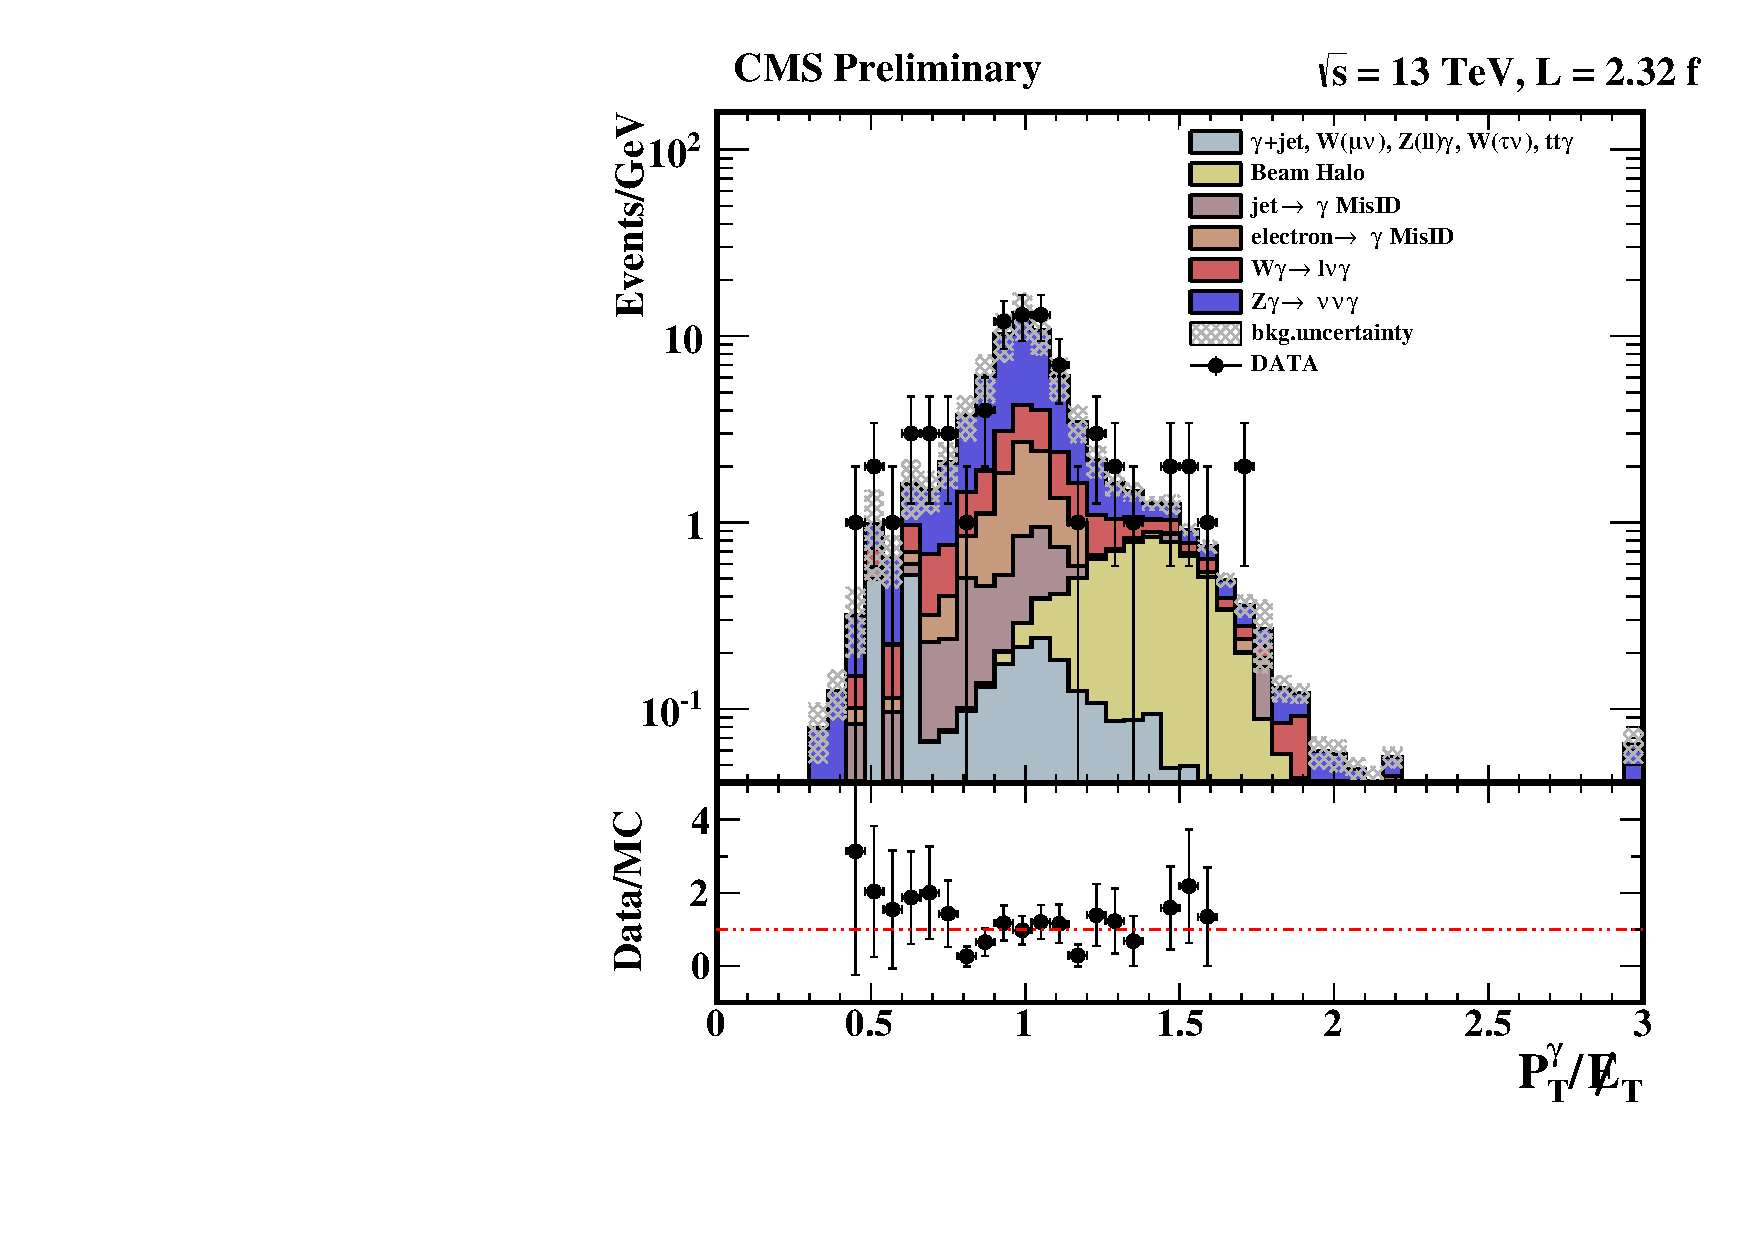
\includegraphics[width=8cm,height=8.0cm]{/Users/rhombus/CMS/Thesis/thesis/pdfs/lgxc/fromb/ptmet8_err.pdf}
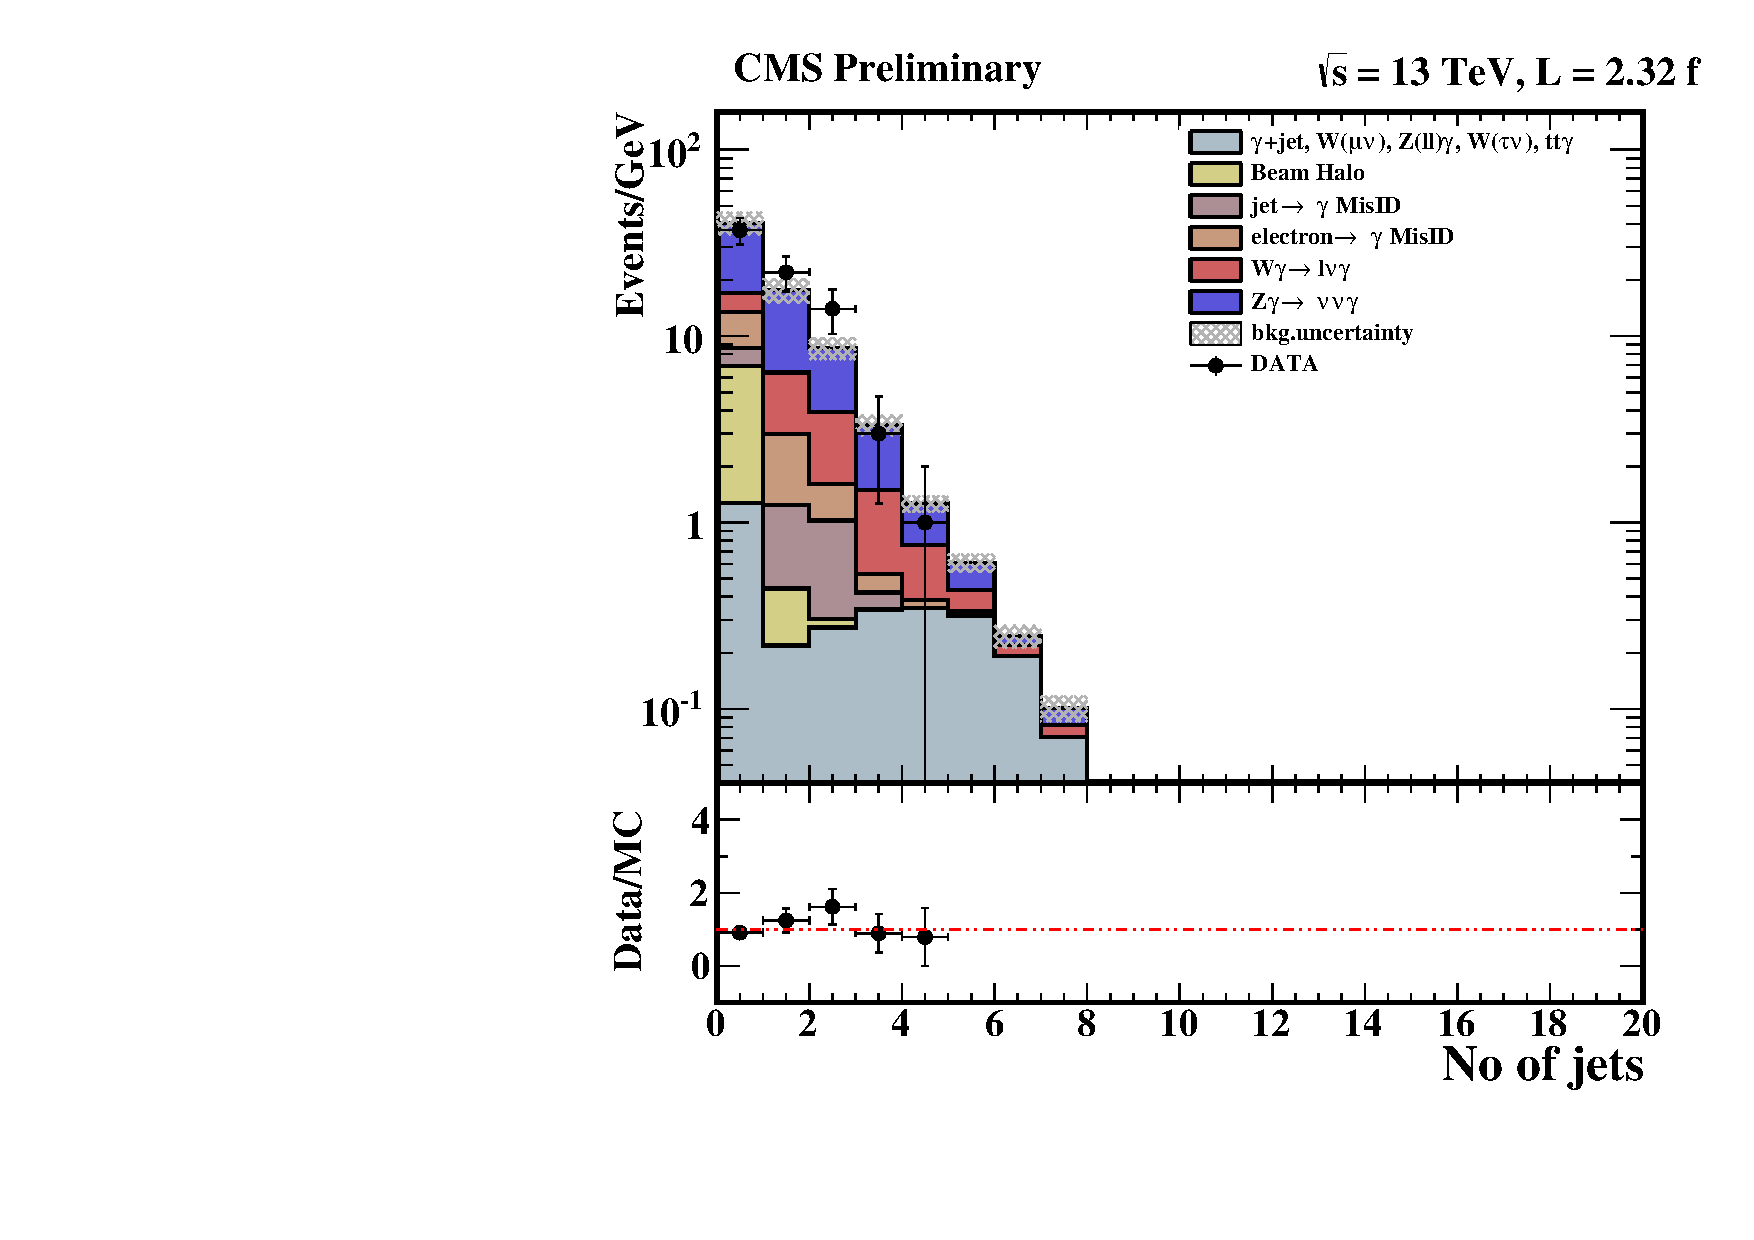
\includegraphics[width=8cm,height=8.0cm]{/Users/rhombus/CMS/Thesis/thesis/pdfs/lgxc/fromb/njet30_err_withdphi.pdf}
\label{fig:ptmetstack1}
\end{figure}



%\begin{table}[htbp]
\begin{table}[!h]
\caption[Estimated yields for \pploneg]
{
 Summary of estimated backgrounds and observed total number of candidates for 2.32 fb$^{-1}$ of 2015 data.
 The category Others includes \wmn, \zllg and \ttg
}
\center
{
\begin{tabular}{c|c}
Process & Estimate \\
\hline
\hline
\zgnng         & 42.10 $\pm$ 6.31   \\
\wglng         & 10.69 $\pm$ 1.49   \\
\wen           & 7.80  $\pm$ 1.78   \\
${jet}\rightarrow\gamma~{fakes}$ & 3.36$\pm$ 1.13 \\
Beam halo      &  5.9 $\pm$  4.7 \\
Others         & 3.05 $\pm$ 0.67  \\
\hline
Total Expectation  &  72.9 $\pm$ 8.30 \\
\hline
Data               & 77    \\
\end{tabular}
\label{tab:BkgSummaryC}
}
\end{table}

\subsection{\ppzgnng Cross Section Measurement}

The  \ppzgnng cross section for $\ptg >175 \GeV$ in the rapidity
 range $\abs{\eta} <$ 1.4 is calculated using the formula

\begin{equation}
 \sigma(\ppzgnng) = \frac{N_{data}-N_{BG}}{A\times\epsilon\times L}
\end{equation}
 where $N_{data}$ is the observed number of events, 
 $N_{BG}$ is the number of estimated background events,
 $A$ is the geometrical and kinematic acceptance of the selection criteria,
 $\epsilon$ is the selection efficiency within the acceptance,
 and $L$ is the integrated luminosity.
%$Br$ is the branching ratio, which in this case is 100\%.
The product of $A\times\epsilon_{MC}$ is estimated from LO \MADGRAPH simulation and a
 correction factor, $\rho$, described in Section \ref{subsubsec:lg_reweighting}
 is applied to account for the difference between the efficiency in the data and 
 Monte Carlo:

\begin{equation}
 A\times\epsilon = A\times\epsilon_{MC} \times \rho  .
\end{equation}

The product of $A\times\epsilon_{MC}$ is estimated to be
 0.314 $\pm$ 0.002 (stat) $\pm$ 0.048 (syst) and rho is 0.99 $\pm$ 0.06.
%Here $A\times\epsilon$ is defined as the ratio of number of events
% passing the full selection to the number of events
% passing  \ptg$ > 175$ \GeV and $\abs{\eta} < 1.4442$.

% and the syst is 7 pecen scale and 6.2 photon/met gives 9%. syst of A*eff 0.0286

The photon energy scale, jet and \met energy scale and resolution,
 and pileup related contributions are considered as
 sources of systematic uncertainty in the acceptance calculation.
The uncertainty on the photon energy scale is about $1.5\%$
 and the uncertainty from variations in the \met energy scales is 5\%.
 %Uncertainties on $\met$ are estimated in accordance to the MET 
 %POG prescription~\cite{met}. 
Contributions from the jet energy scale are accounted for in the  uncertainty on  
the \met. 
The uncertainty on the integrated luminosity is 2.7$\%$~\cite{LUM-13-001}.
A summary of the systematic uncertainties are shown in Table ~\ref{tab:sysfull1}.

\begin{table}[htbp]
\centering
{\scriptsize
\resizebox {\textwidth }{!}{ % 
\begin{tabular}{|c|c|c|c|c|c|c|}
\hline
Sources & \zgnng [\%] & \wglng [\%] & Jets faking photon [\%] & Electron faking photon & gamma-jet & Other bkgs [\%] \\
\hline
Luminosity & 2.7    & 2.7  & - & - & 2.7 &  2.7 \\
\hline
PDF and Scale & 5.37 & 8.9 & - & -& -& -\\ 
\hline
EWK corrections &  11 & 7 & - & - & - & -\\ 
\hline
Jets faking photon & - & - & 30 & - & - & -\\ 
\hline
Elecron faking photon & - & -& -& 20 & - & -\\ 
\hline
Jet, MET, photon energy scale &  6 & 6 &-& - & 6 & 6\\ 
\hline
Scale Factors & 6 & 6 & -& - & 6 & 6\\ 
\hline

\end{tabular}}
\caption{Summary of systematic unceratinties for signal and different background sources.}
\label{tab:sysfull1}}
\end{table}

The measured cross section for \ppzgnng  for photon $p_T >$ 175 GeV within
 rapidity range $\mid \eta_{\gamma}\mid < $1.4
 is 
\begin{equation}
 64.06 \pm 12.14({stat.}) \pm 12.88({sys.}) \pm 1.72({lumi.}) \fb.
\end{equation}
The NNLO therotical cross section is $65.55\pm 0.02$ \fb
  where the uncertainty includes only the scale variaitons. 
The measured cross section agrees well with the NNLO theoritical cross section
 and this agreement with the SM prediction constrains
 possible DM models.

 \subsection{Limits on Dark Matter}
\label{ssec:lim_DM}
Interpreting these results as setting limits on the
 cross section of a DM particle as a function of 
 DM mass, Tables~\ref{table:vxslimits} and \ref{table:avxslimits}
 show 90\% confidence level (CL) upper limits on the
 production cross sections provided infor the Vector
 and the Axial-vector model for a mediator mass of 10 \TeV. 
%Using a type-I error rate ($\alpha$) of 0.10 instead of the ``industry standard'' 0.05 used in exotic searches because we want to compare our results against other experiments for which $\alpha=0.10$ is considered standard.
%We are working on other mass points for the dark matter and will present results soon.


\begin{table}[ht]
\centering
\begin{tabular}{cc}
\hline\hline
Mass DM [GeV] & $\sigma$ [fb] \\
\hline
1  & 3.821(3.242)  \\  
\hline
10  & 3.820(3.244)  \\  
\hline
50  & 3.827(3.249) \\
\hline
150  & 3.826(3.254)\\
\hline 
500  & 3.588(3.052) \\
\hline
1000  & 3.370(2.862) \\
\hline
\end{tabular}
\caption{Observed (expected) 90\%CL upper limits on the dark-matter production cross section $\sigma$ for mediator mass 10 TeV. }
\label{table:vxslimits}
\end{table}



\begin{table}[ht]
\centering
\begin{tabular}{cc}
\hline\hline
Mass DM [GeV] & $\sigma$ [pb] \\
\hline
1  & 3.782(3.211)  \\  
\hline
10  & 3.785(3.213) \\
\hline
50  & 3.793(3.213) \\
\hline
150  & 3.754(3.192)\\
\hline
500  & 3.488(2.961)\\
\hline
1000  & 3.30(2.814)\\
\hline
\end{tabular}
\caption{Observed (expected) 90\%CL upper limits on the dark-matter production cross section $\sigma$ for fixed mediator mass 10 TeV }
\label{table:avxslimits}
\end{table}





